\section{Proof of the five colour theorem}
In order to prove Theorem~\ref{thm:five_colour}, we restate it as a Proposition, on which we can perform induction:
\begin{proposition}[Five colour theorem]
\label{prop:five_colour}
A graph $G_n = (V, E)$, which is planar-connected with n vertices and m edges, is 5-colourable $\forall n \in \mathbb{N}^{>0}$
\end{proposition}

We proceed by induction on $n$:
\begin{proof} Let Proposition~\ref{prop:five_colour} be labeled $\prop{n}$ \vspace{.1cm} \\
\textbf{Base case}: \textit{Show that $\prop{n}$ holds for $1 \leq n \leq 5$} \\
test \vspace{.1cm} \\
\textbf{Induction hypothesis}: \textit{Assume $\prop{n}$ holds for $n \geq 5$, show that $\prop{n + 1}$ follows} \vspace{.1cm}

We assume that $G_{n}$ is 5-colourable, and we need to inductively show that the same is true for $G_{n + 1}$ \vspace{.1cm} \\
\textbf{Induction step}: \textit{Prove $\prop{n + 1}$} \vspace{.1cm}

By Lemma~\ref{lem:deg_leq_six}, $\exists v \in V(G_{n + 1})$ such that the $\deg(v) < 6$. For the sake of the proof, let us construct $H_{n} \defeq G_{n + 1} \setminus \{v\}$ where $\deg(v) = 5$. By the hypothesis, $H_{n}$ is 5-colourable. The goal is to show that based on our construction of $H_{n}$, that $H_{n} \cup \{v\} \eqdef G_{n + 1}$ is always 5-colourable. Let us consider the neighbourhood of $v$ (which are all the adjacent vertices of $v$) and denote it as $N(v) = \{v_1, v_2, v_3, v_4, v_5\} \subseteq H_{n}$. We define the 5-colouring of the graph $H_n$ as $c : V(H_{n}) \longrightarrow \{i \in \mathbb{N} : 1 \leq i \leq 5\}$. By our assumption, $N(v) \subseteq V(H_{n})$ admits either 5 or less than 5 colours, therefore: \\
\textbf{case 1}: $|\{c(v_{i}) : v_{i} \in N(v)\}| < 5$

Let $G_{n + 1} \defeq H_{n} \cup \{v\}$ and $c(v) \defeq k$, where $k \in \{ c(v_{i}) \}_{v_{i} \in H_{n}} \setminus \{ c(v_{i}) \}_{v_{i} \in N(v)}$ i.e $v$ gets assigned any remaining colour and we are done

\begin{figure}[H]
\centering
\begin{subfigure}[H]{0.49\textwidth}
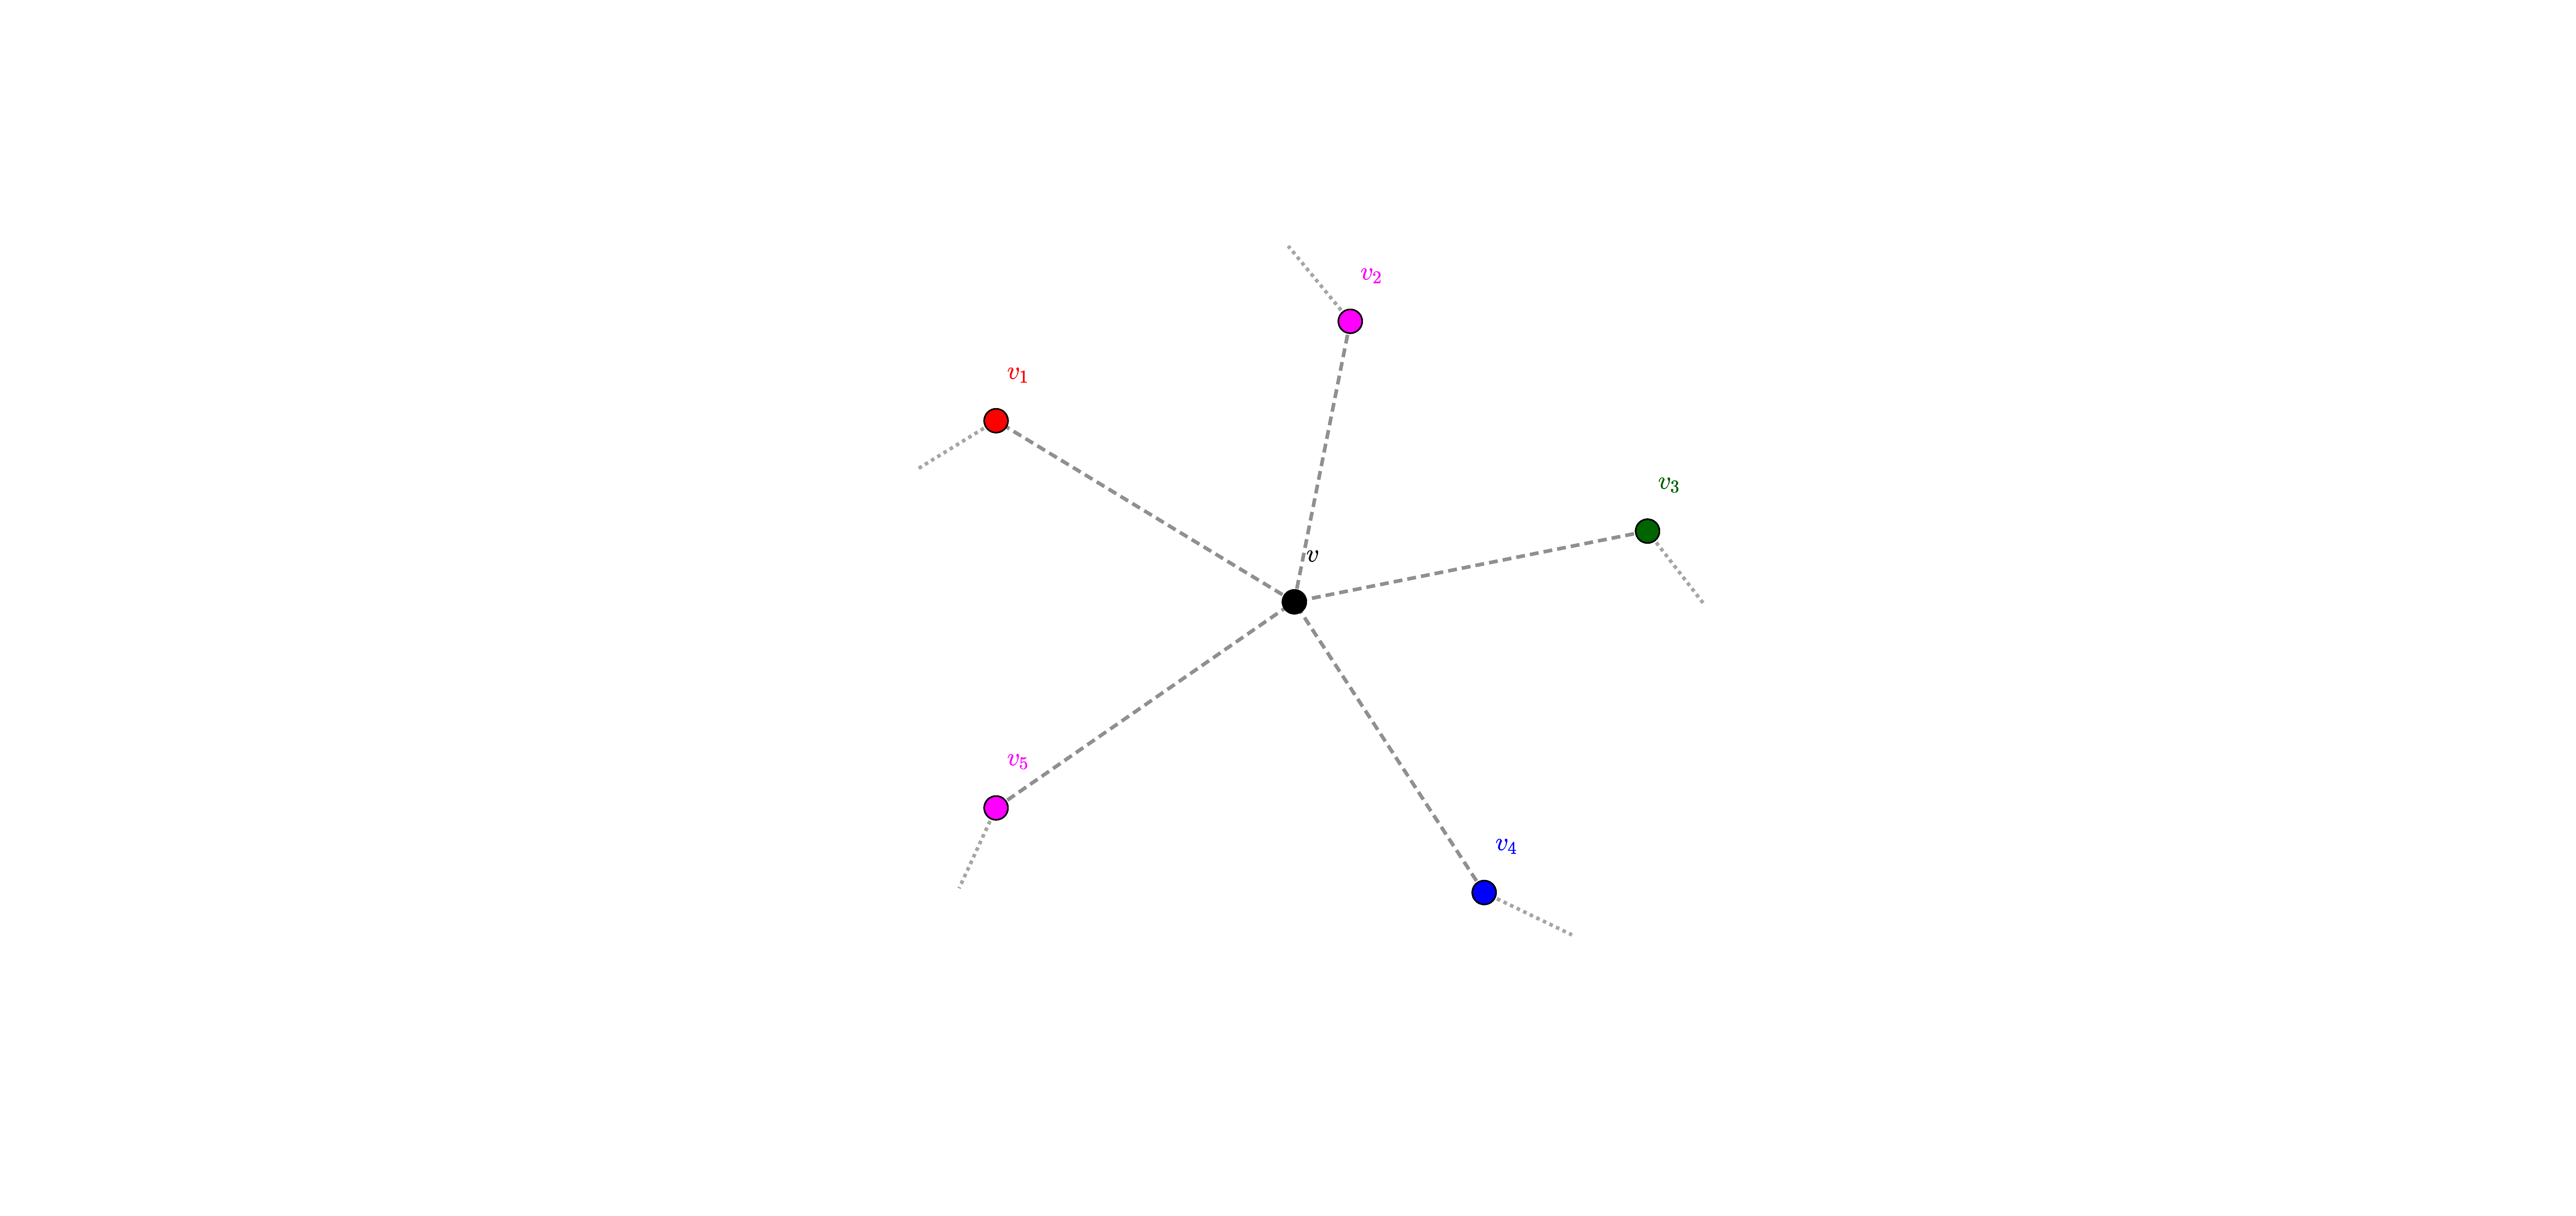
\includegraphics[width=\textwidth]{img/case1_first.pdf}
\caption{Diagram of $N(v) \subseteq H_{n}$}
\label{fig:case1_first}
\end{subfigure}
\begin{subfigure}[H]{0.49\textwidth}
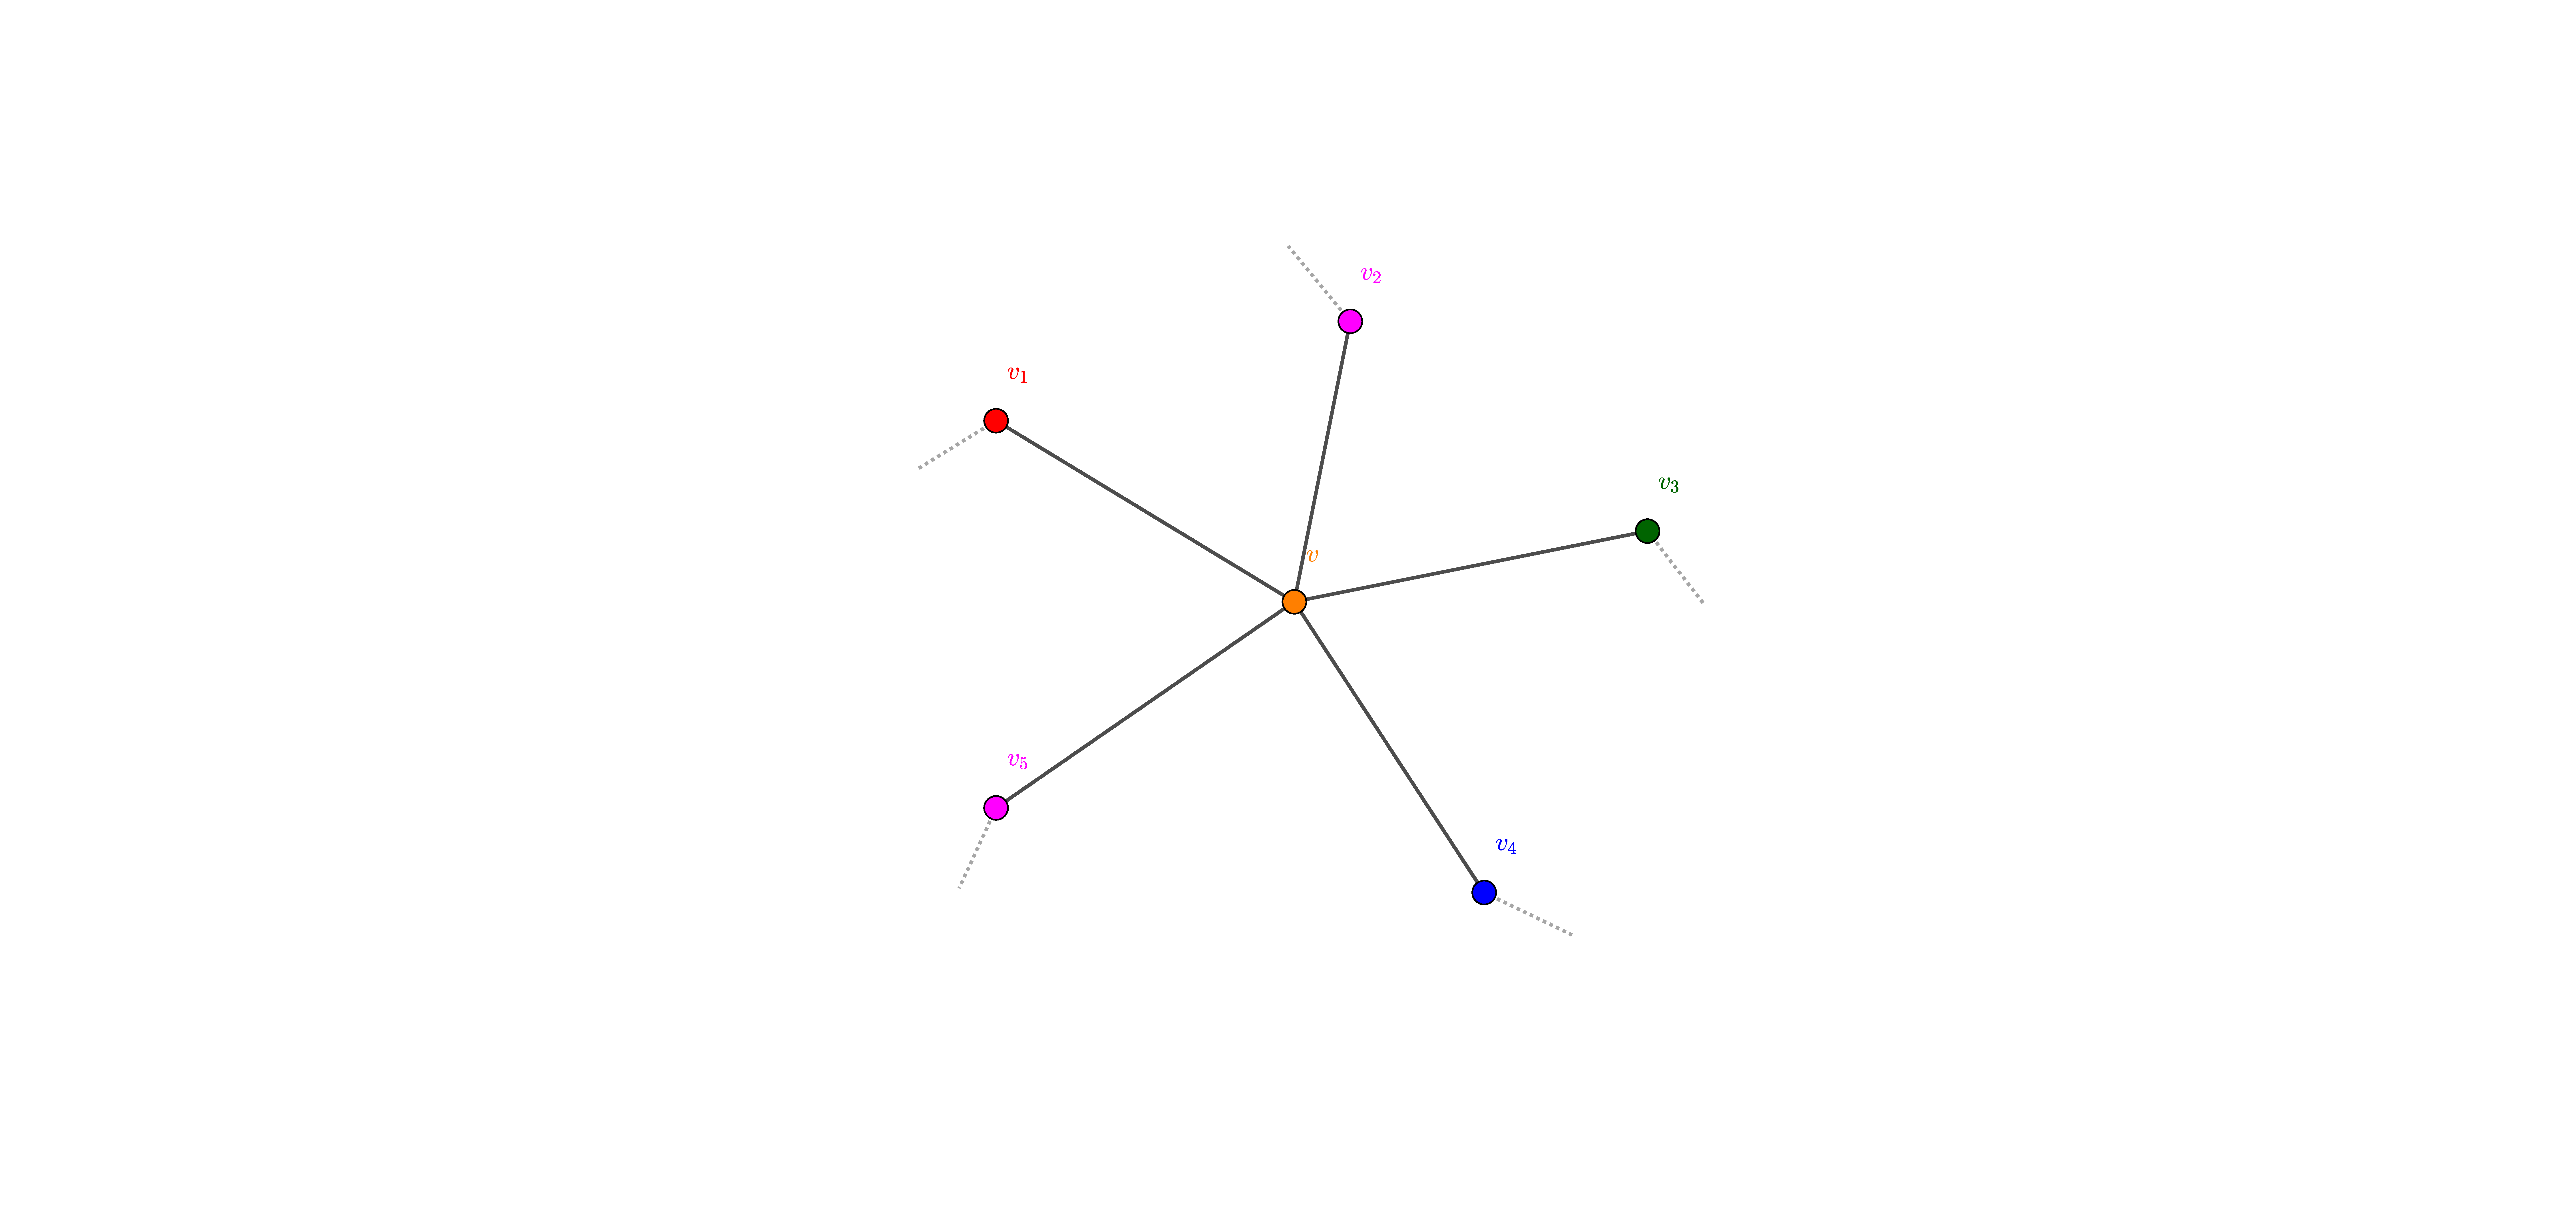
\includegraphics[width=\textwidth]{img/case1_second.pdf}
\caption{Diagram of $N(v) \subseteq G_{n + 1}$}
\label{fig:case1_second}
\end{subfigure}
\caption{Graph focussed around $N(v)$. The dotted lines represent arbitrary edges, whereas the vertices connected by the dashed edge are disjoint}
\end{figure}

$\phantom{x}$ \\
\textbf{case 2}: $|\{c(v_{i}) : v_{i} \in N(v)\}| = 5$

Since all vertices of $v$ are uniquely coloured, we cannot construct $G_{n + 1}$ such that it has a 5-colouring. We must reduce the colouring of $H_{n}$ so $v$ can be assigned the missing colour. For this let us consider a subgraph $H_{i, j} \subset H_{n}$, where $c(v_{i})$ and $c(v_{j})$ are the only possible colourings. This allows us to generalise the graph in such a way that vertices can be assigned different colours while maintaining a 5-colouring. Let us arbitrarily consider the vertices $v_{1}$ and $v_{3}$ from the previous illustration with $H_{1, 3} \subset H_{n}$. We now consider two more cases: \\
\textbf{case 2a}: Suppose $v_1$ and $v_3$ are not connected by a path in $H_{n}$

All vertices $v_i, v_j \in V(H_{i, j})$ where $c(v_i) \not = c(v_j)$ can be swapped with respect to each other without the need to modify the colouring of any other vertices outside of $H_{i, j}$. Since both $v_1, v_3 \in V(H_{1, 3})$, we are allowed to set $c(v_1) \defeq c(v_3)$ (or vice versa), such that $G_{n + 1} \defeq H_{n} \cup \{v\}$ and $v$ gets assigned the missing colour (as explained in case 1).

\begin{figure}[H]
\centering
\begin{subfigure}[H]{0.49\textwidth}
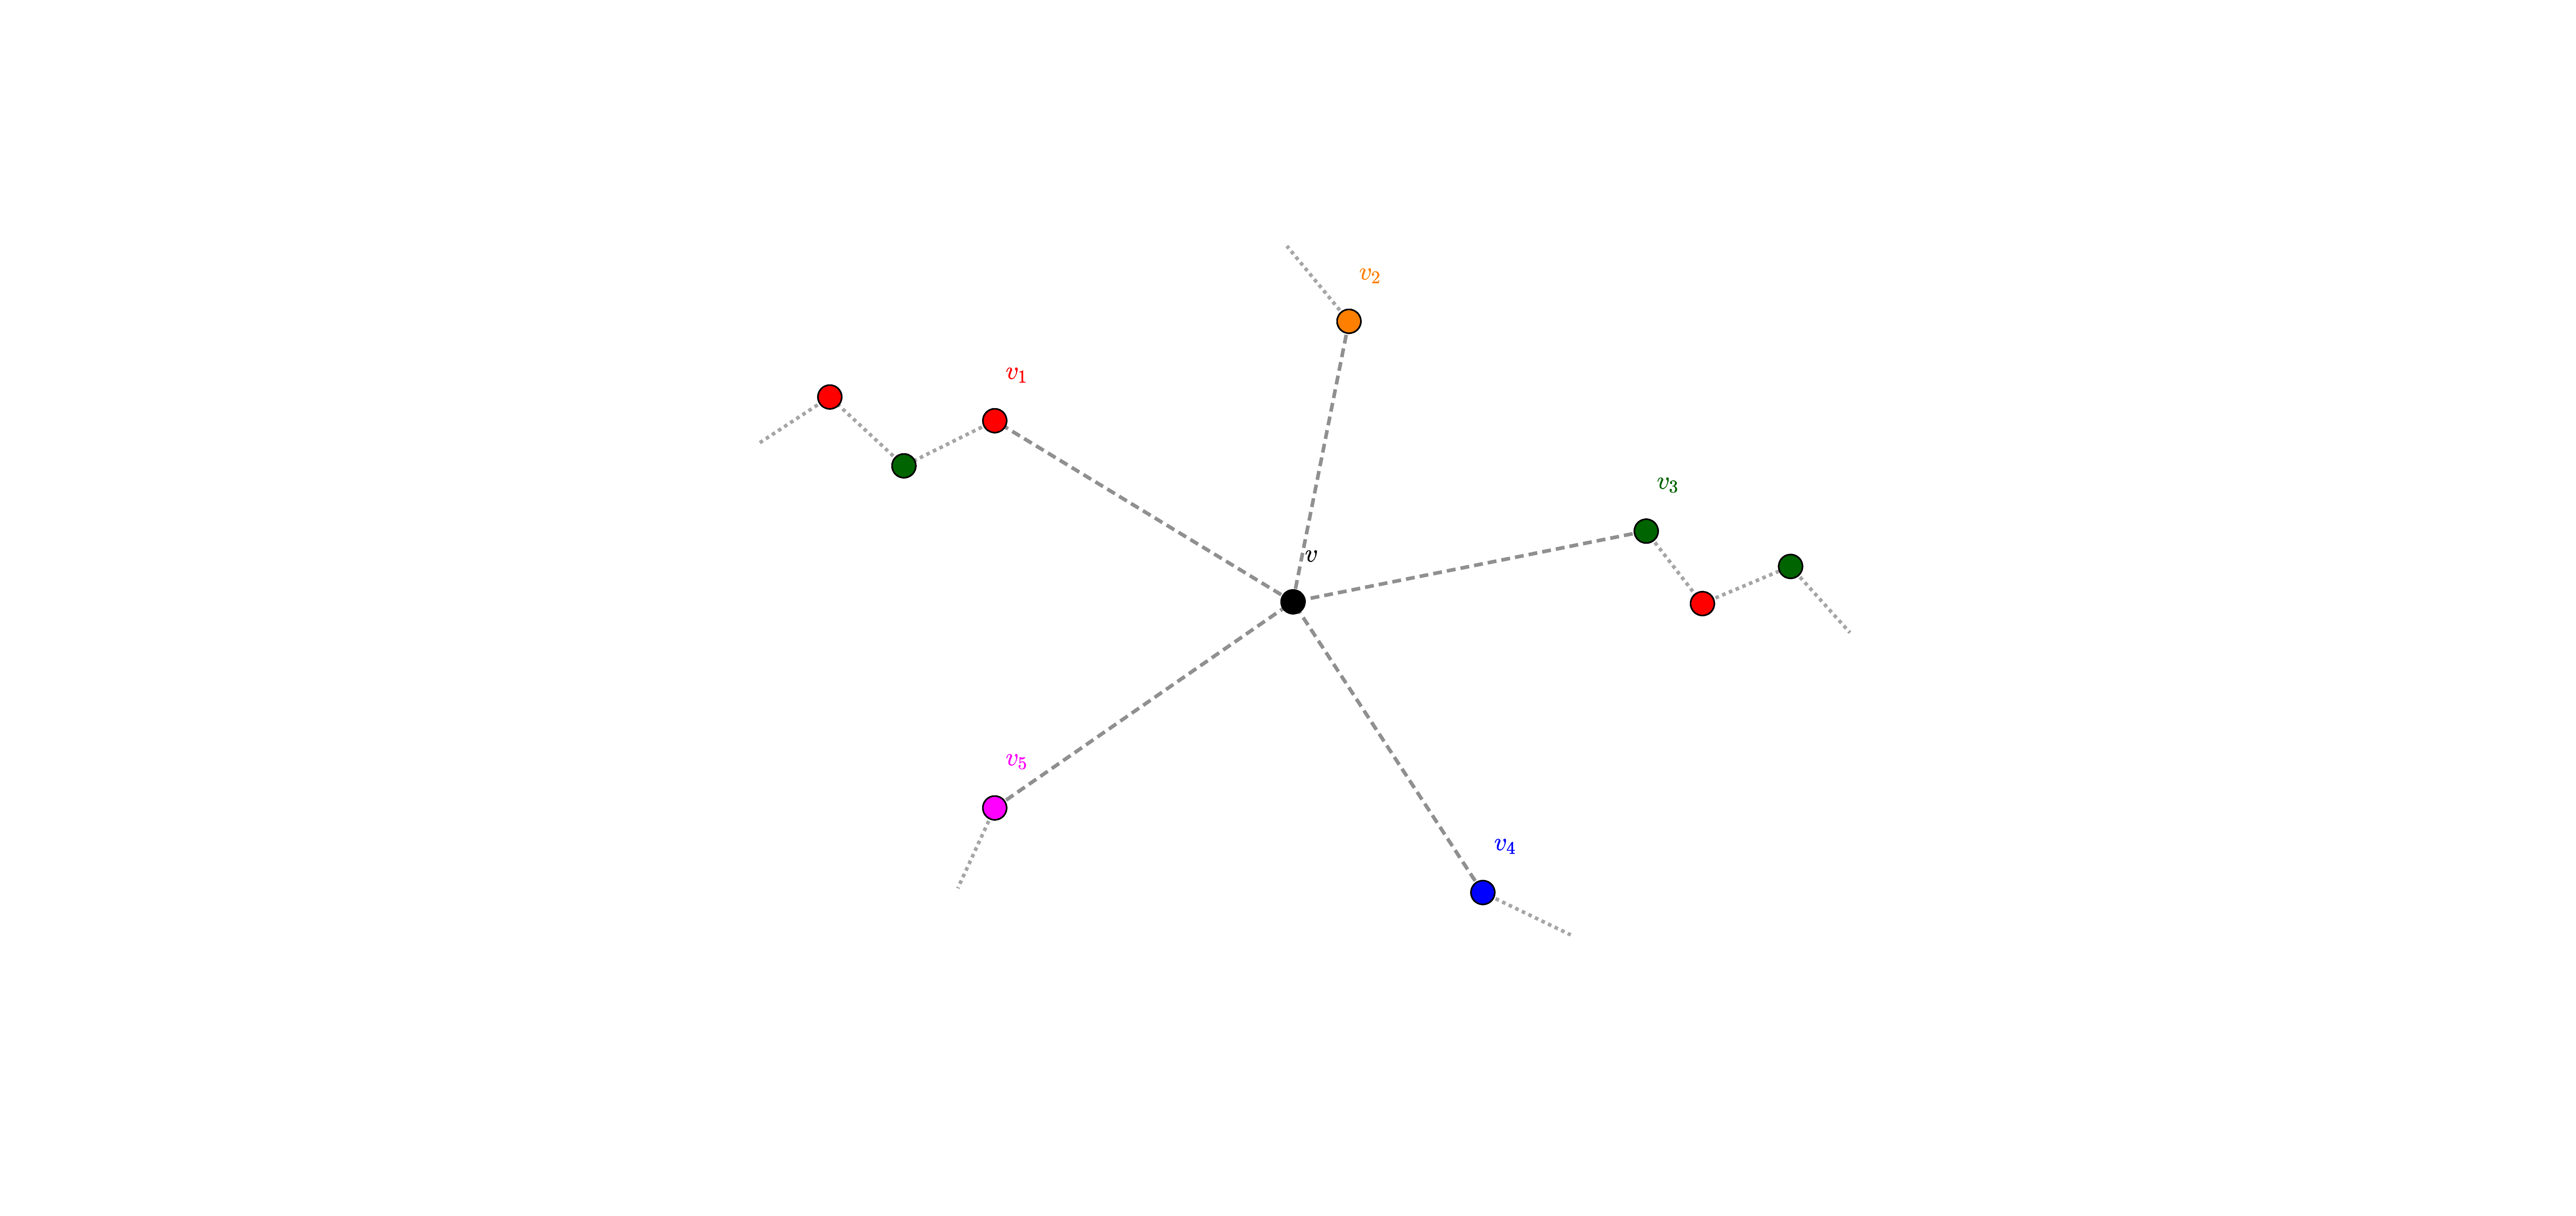
\includegraphics[width=\textwidth]{img/case2a_first.pdf}
\caption{Diagram of $N(v) \subseteq H_{n}$}
\label{fig:case2a_first}
\end{subfigure}
\begin{subfigure}[H]{0.49\textwidth}
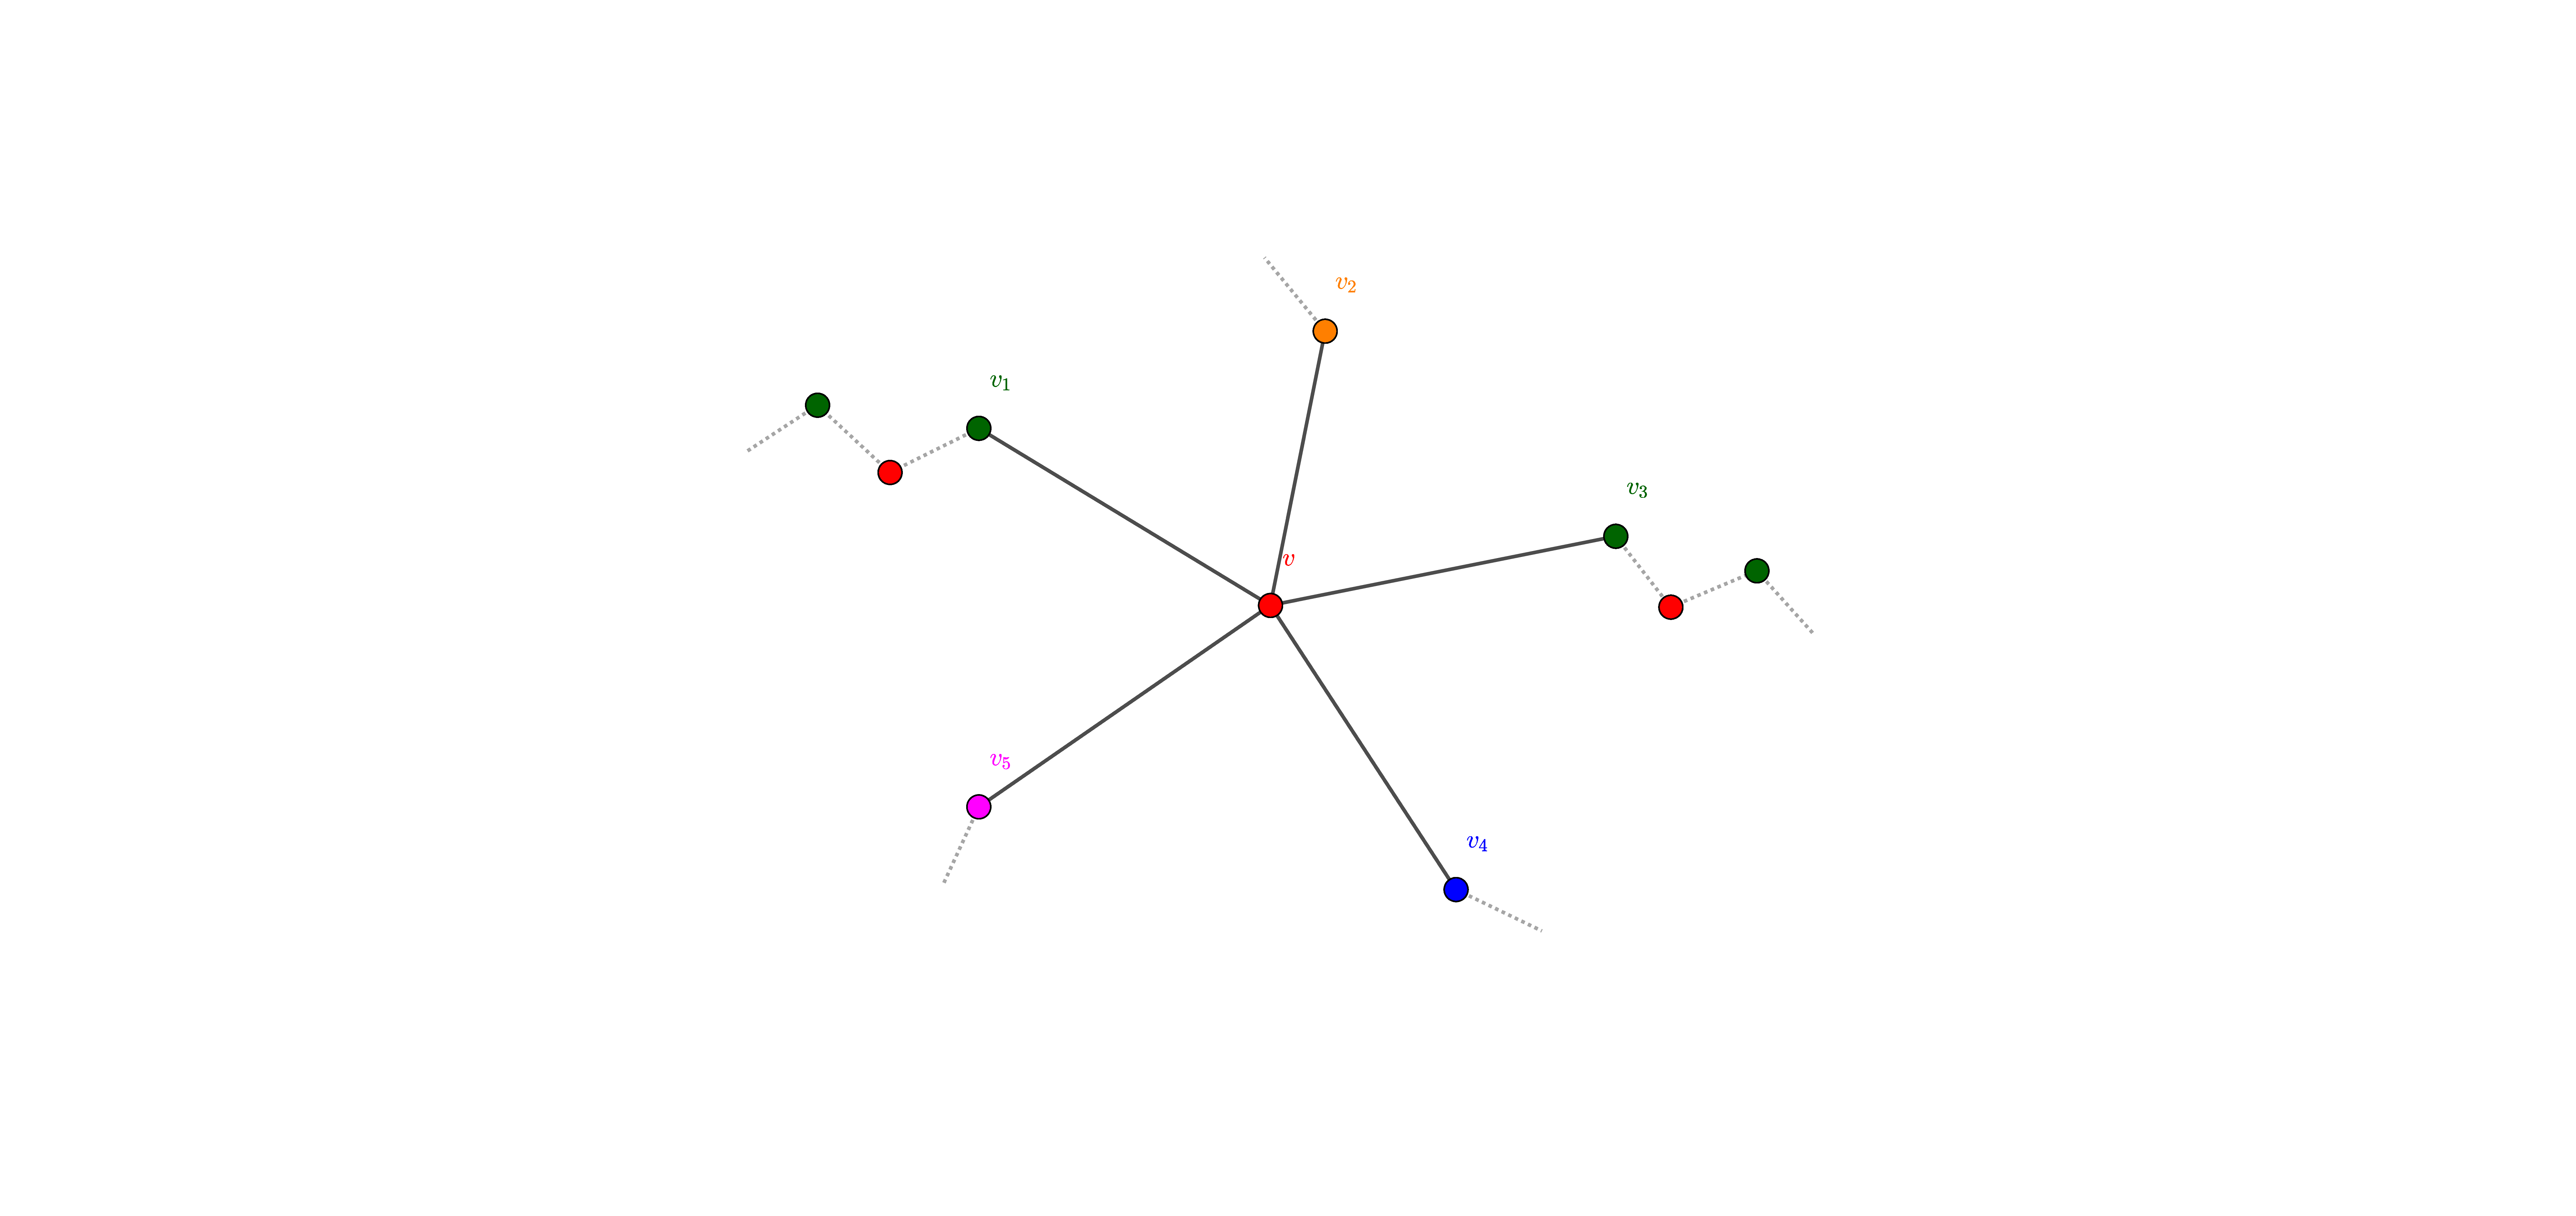
\includegraphics[width=\textwidth]{img/case2a_second.pdf}
\caption{Diagram of $N(v) \subseteq G_{n + 1}$}
\label{fig:case2a_second}
\end{subfigure}
\caption{Comparison of the planar graph before and after recolouring and union of $v$}
\end{figure}

$\phantom{x}$ \\
\textbf{case 2b}: Suppose $v_1$ and $v_3$ are connected by a path in $H_{n}$

Here the path of vertices connecting $v_{1}$ and $v_{3}$ in $H_{1,3} \cup \{v\}$ forms a cycle which contains $v_{2}$. We can safely assume that by our construction of $H_{1,3}$, the vertices $v_{2}$ and $v_{4}$ cannot be connected by a path in $H_{2,4}$, since this would disrupt the planarity of the graph $H_{n}$ (by intersecting edges). Because of this, $c(v_{2}) \defeq c(v_{4})$ (as in case 2a). Therefore $G_{n + 1} \defeq H_{n} \cup \{v\}$ and $v$ gets assigned the missing colour.

\begin{figure}[H]
\centering
\begin{subfigure}[H]{0.49\textwidth}
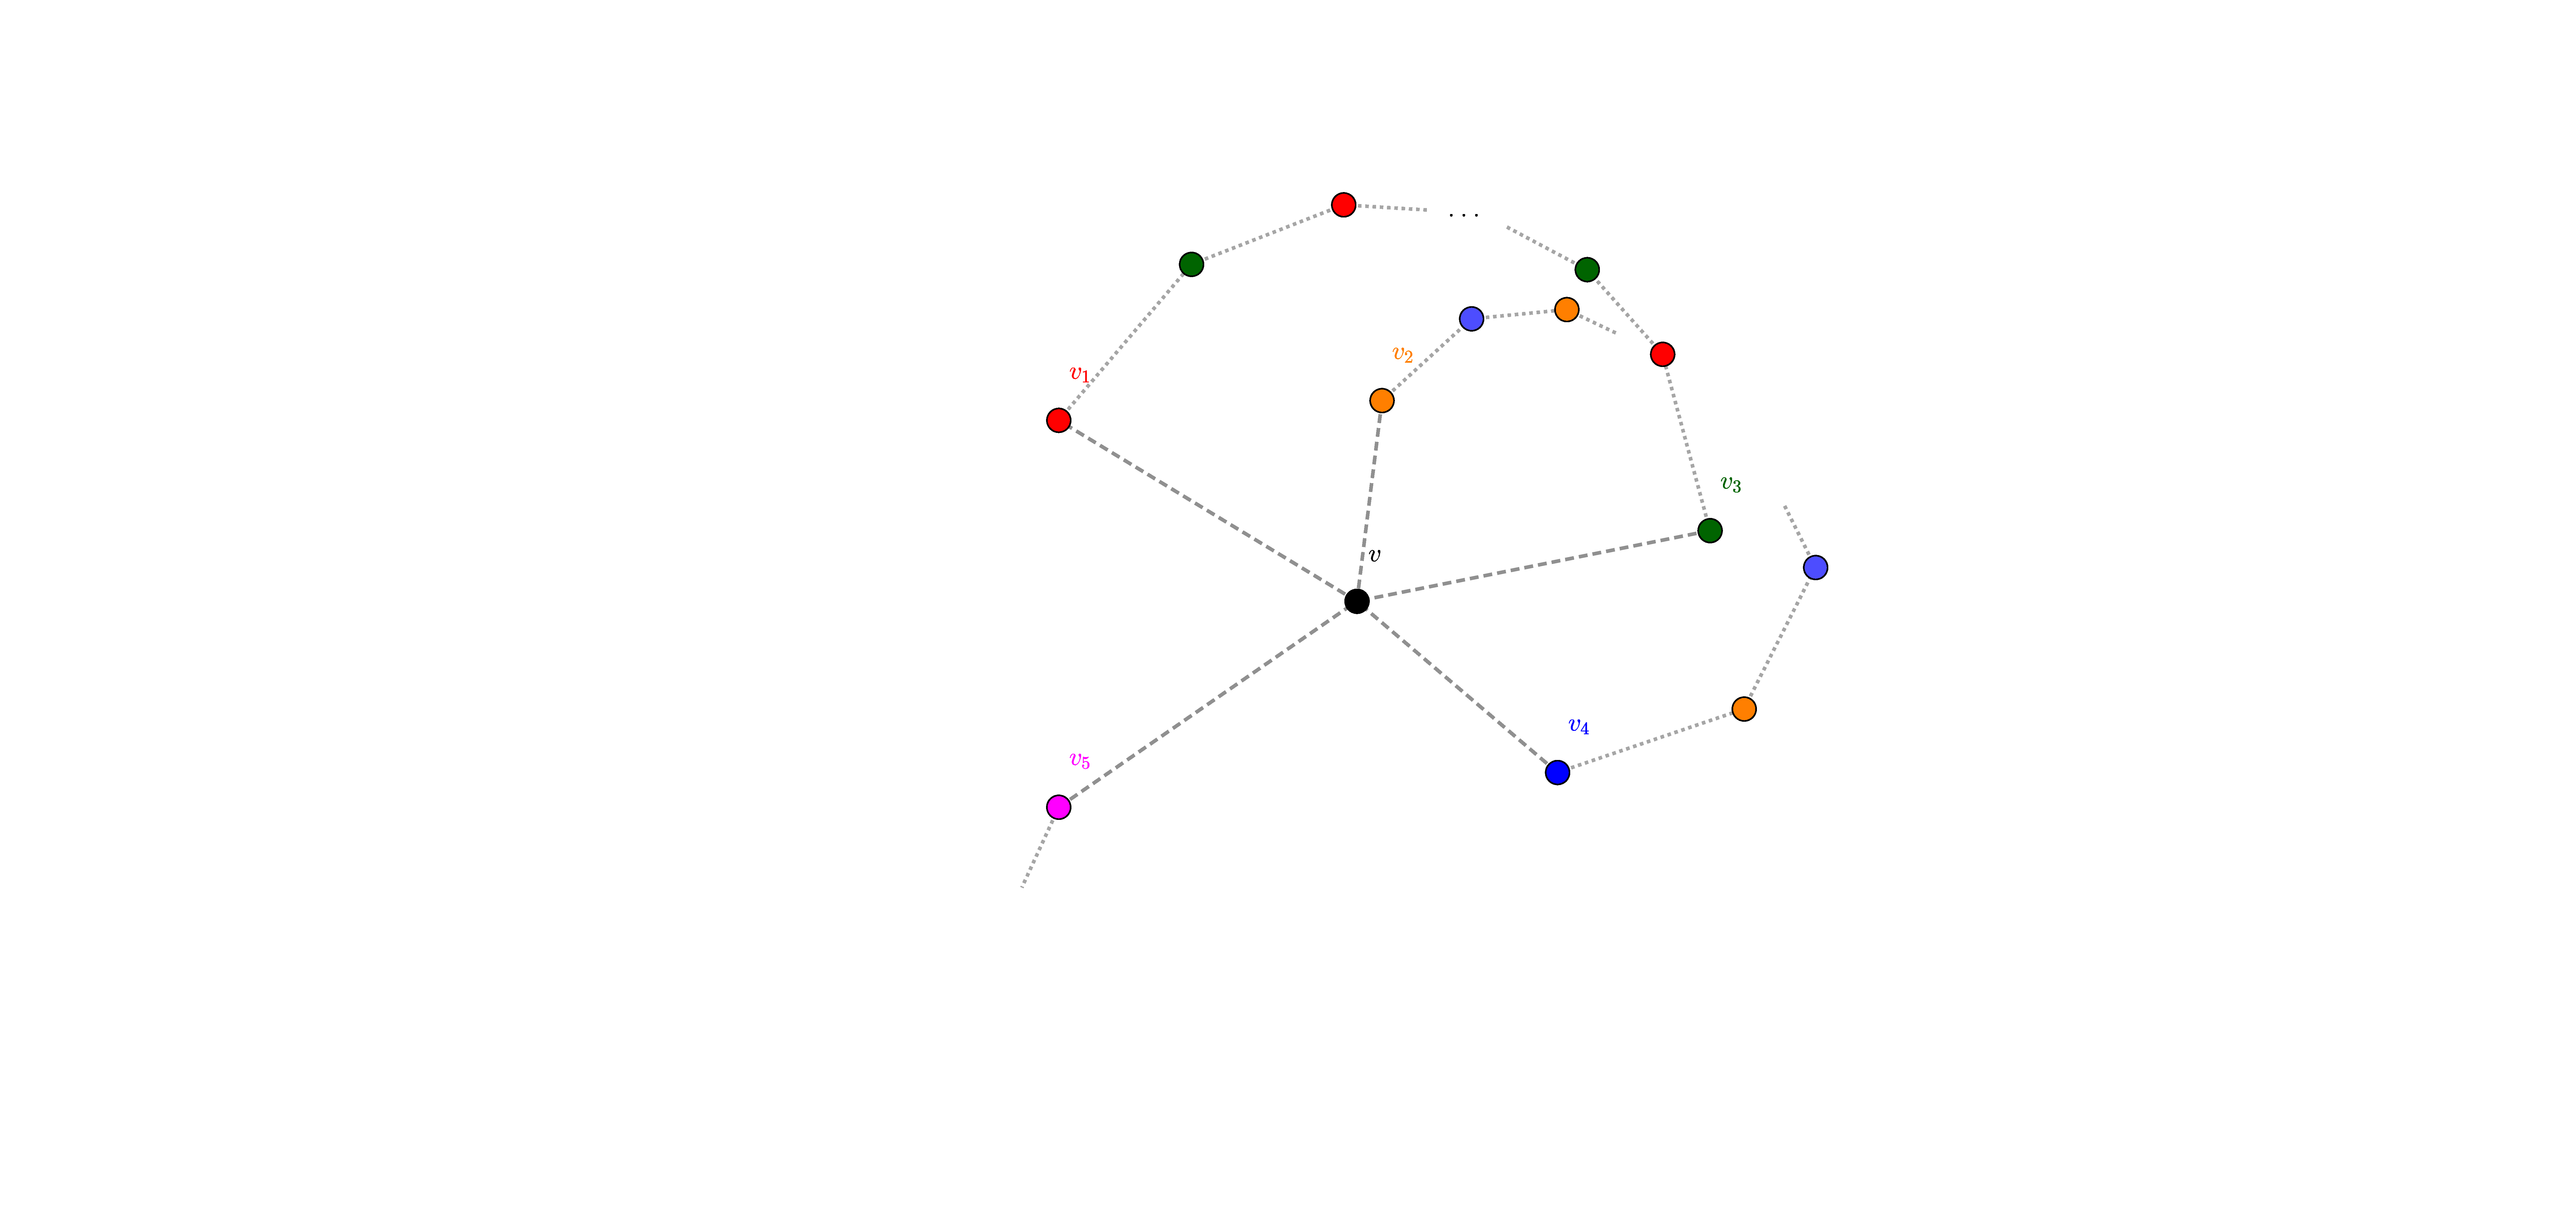
\includegraphics[width=\textwidth]{img/case2b_first.pdf}
\caption{Diagram of $N(v) \subseteq H_{n}$}
\label{fig:case2a_first}
\end{subfigure}
\begin{subfigure}[H]{0.49\textwidth}
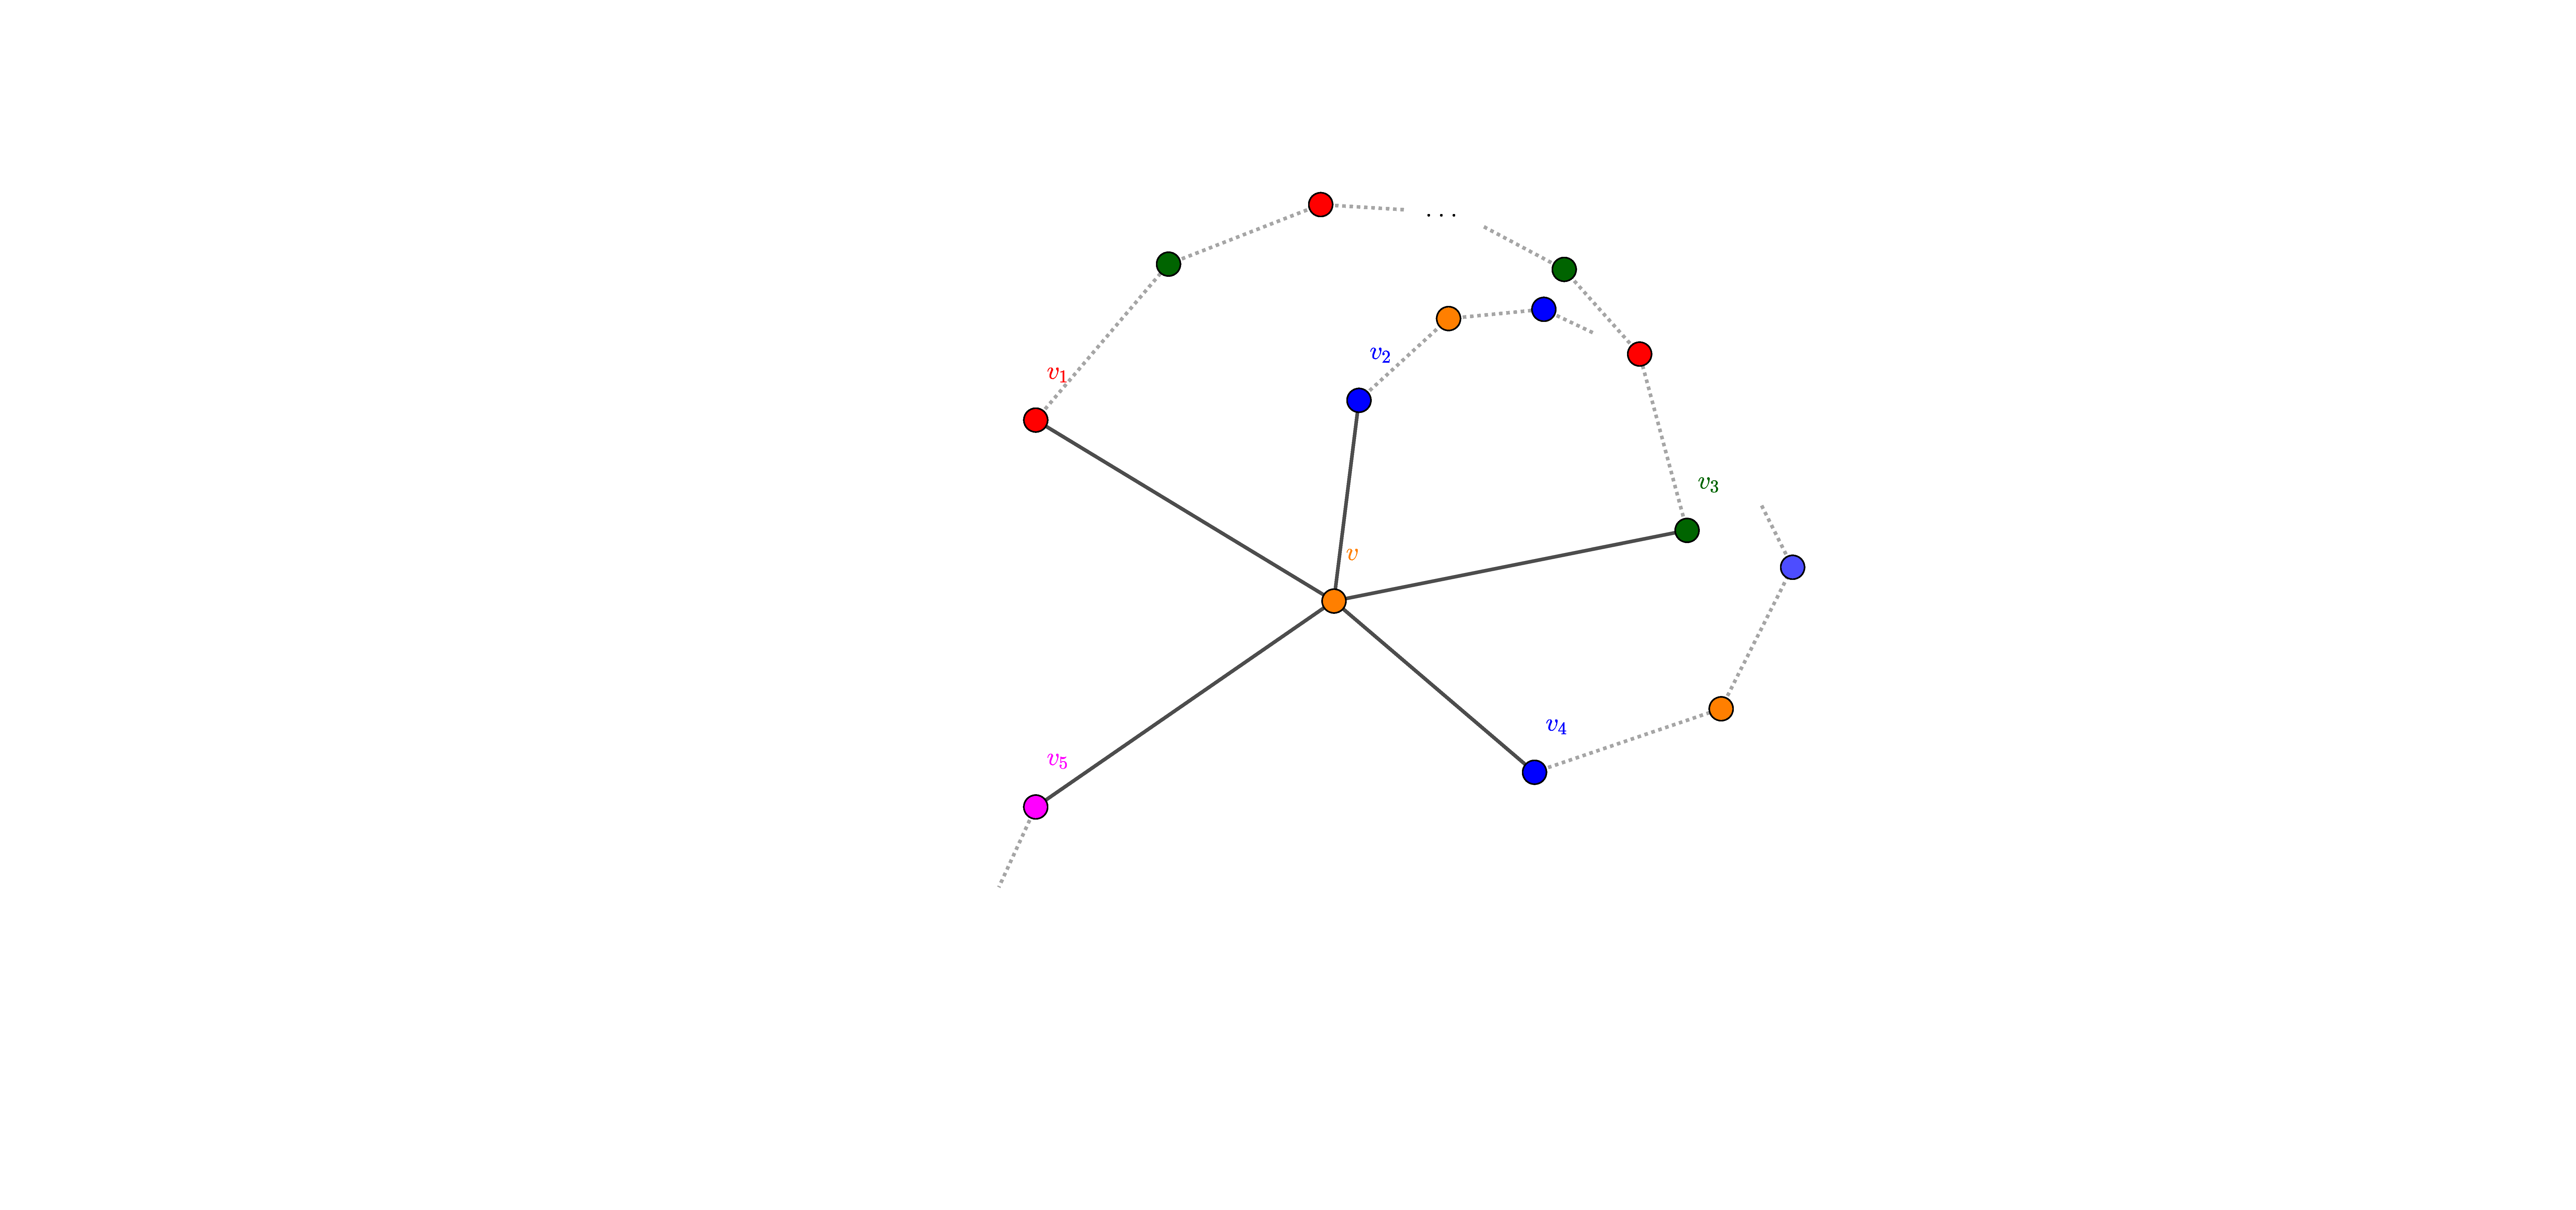
\includegraphics[width=\textwidth]{img/case2b_second.pdf}
\caption{Diagram of $N(v) \subseteq G_{n + 1}$}
\label{fig:case2a_second}
\end{subfigure}
\caption{Comparison of the planar graph before and after recolouring and the union of $v$}
\end{figure}

Since we can always find a way to recolour $H_{n}$ so that $H_{n} \cup \{v\} \eqdef G_{n + 1}$ is 5-colourable, by the principle of mathematical induction, $G_{n}$ is 5-colourable $\forall n \in \mathbb{N}$
\end{proof}